\chapter{Experiments}

This chapter deals with discussing the experiment performed with different models to classify stereotypical social biases using the stereotypical dataset discussed in the previous section. Section \ref{task_overview} describes the basic overview of the classification task, with some insights into the data. Section \ref{experimental_setup}  discusses the basic setup for performing experiments. Section \ref{assessing_social_biases} describes the language models and baselines used, along with the training procedure. Finally, \ref{evaluation_metrics} describes about the evaluation metrics used when assessing the results.

\section{ Task overview}\label{task_overview}
The main goal of the thesis is to assess social stereotypes present in the text sequences using language models. The reasons for using language models which is based on transfer learning approach are as follows, firstly, when training a model using the classic supervised learning approach, where in, a model is trained on a dataset belonging to the source domain with training samples that demonstrate correct behavior and then tested on an identically distributed held out samples, the model tends to perform well \cite{ruder2019neural}. Moreover, these models require several hundred to thousands of samples to induce functions which generalize well \cite{radford2019language}. This approach might not suite for the task of assessing social stereotypes as the number of samples are relatively less. Transfer learning approach on the other hand is more preferable for the current setting where in the knowledge gained through training on the source domain/task is stored as representations (vectors) and applied to target domain or task \cite{ruder2019neural} rather than training from scratch as done in classic supervised learning approach. Transfer learning in the form of pretrained language models have become ubiquitous in natural language processing and contributed to state of the art on a wide range of tasks\cite{ruder2019transfer}. Due to the fact that the pre-trained language models have been trained on large amounts of real world data, the need for annotated data is reduced by 10x. Transfer learning using pre-trained language models have been shown to achieve similar performance compared to non-pretrained model with 10x fewer samples \cite{howard2018universal}. During this pre-training, they also capture the stereotypical biases present in the data \cite{nadeem2020stereoset}. This knowledge can thus be used for the target task of classifying stereotypical social biases. Considering these reasons, experiments have been performed on different pretrained language models. In order to evaluate the performance of language models and to answer the second research question of how far transfer learning can be used to detect stereotypes, baselines have been trained, which will be discussed in the corresponding section.

Considering the task of classification, several experiments using different combination of labels (stereotype, anti-stereotype, different bias types) and different classification tasks (binary, multi-class, multi label) have been performed to test the different perspectives of predictions. Finally, multi label classification was chosen with ethnicity, gender, profession, religion, stereotype, anti-stereotype, unrelated as labels. Considering the datasets stereoset and crowspair, as can be seen in the table \ref{tab:stereoset} and \ref{tab:Crowspair}, for each bias type there is a stereotypical as well as anti-stereotypical instance. Considering the perspective that stereotypes only have meaning to the extent they are socially shared \cite{macrae1996stereotypes}, anti-stereotype samples gives the perspective that the sample is a stereotype but not socially shared. Hence, considering anti-stereotype along with stereotype as a label gives the perspective whether a sample is socially share or not socially shared stereotype. To put it more clearly, stereotype samples are socially shared stereotypes, while anti-stereotypes are not socially shared stereotypes. Stereoset dataset also contain an unrelated instance per sample, this instance can be used as a sample which is neither socially shared (stereotype) nor not socially shared (anti-stereotype) but a totally unrelated sample. Hence, to the pre-processed dataset \ref{tab:Bias_type_stats_preprocessing}, anti-stereotypical samples from stereoset (combining context and anti\_stereotype instance ; see table \ref{tab:stereoset} for reference) and crowspair (sent\_less of crowspair; see table \ref{tab:Crowspair} for reference) are added. Stereoset Unrelated intersentence samples are added, excluding intrasentence unrelated. Considering the intrasentence stated in the table \ref{tab:stereoset}, the unrelated instance would be "girls tend to be more \textit{fish} than boys" which does not make any sense and thus are omitted. Data augmentation technique is used to generate unrelated synthetic samples using NLPaug \footnote{\url{https://github.com/makcedward/nlpaug}} library. The unrelated samples of intersentence were used as reference to generate synthetic samples by substituting certain number of words (word augmenter). contextual word embeddings of roberta-base model is used to substitute the original word in the reference sentence using similarity measure between original word and the word embeddings of the model. Hence, the final dataset statistics after adding anti-stereotypical samples and unrelated samples are as shown in the figure \ref{tab:data_final_stats}.

% Please add the following required packages to your document preamble:
% \usepackage{booktabs}
% \usepackage{graphicx}
\begin{table}[]
\centering
\scalebox{0.3}{
\resizebox{\columnwidth}{!}{%
\begin{tabular}{@{}lr@{}}
\toprule
Biat type             & No. of samples             \\ \midrule
Ethnicity             & 5226                       \\
Profession            & 3112                       \\
Gender                & 2024                       \\
Religion              & 1953                       \\\bottomrule
\addlinespace
Total                 & 16560 \\ \bottomrule
% \multicolumn{1}{l|}{Total} & \multicolumn{1}{|l}{16560} \\ \bottomrule
\end{tabular}%
}}
\caption{Data statistics after combining anti-stereotypical and unrelated samples}
\label{tab:data_final_stats}
\end{table}


% Please add the following required packages to your document preamble:
% \usepackage{booktabs}
% \usepackage{graphicx}
\begin{table}[]
\resizebox{\textwidth}{!}{%
\begin{tabular}{@{}llllllll@{}}
\toprule
Ethnicity & Gender & Profession & Religion & Anti-stereotype & Stereotype & Unrelated & Sentence                                                         \\ \midrule
1 & 0 & 0 & 0 & 0 & 1 & 0 & Many people live in Ethiopia. The people are very thin and good at distance running \\
1         & 0      & 0          & 0        & 1               & 0          & 0         & Many people live in Ethiopia. The people are fat and unatheletic \\
0         & 0      & 0          & 0        & 0               & 0          & 1         & I saw a cowboy                                                   \\ \bottomrule
\end{tabular}%
}
\caption{One hot encoded stereotypical dataset }
\label{tab:ohe_df}
\end{table}

As shown in the table \ref{tab:ohe_df}, the final dataset consists of one hot encoded vectors where for each sample of stereotype (socially shared) or anti-stereotype (not socially shared), a corresponding bias type i.e. either ethnicity, gender, profession or religion is also present. This categorization thus answers whether a sample is a socially shared stereotype or not along with the bias type or its a totally unrelated sample.
% \begin{itemize}
%     \item Why transfer learning based approach ?
%     \begin{itemize}
%         \item Less number of samples available due to the multidimensional nature of stereotypes, and collecting and validating stereotypes is not a straight forward task.  
%         \item Use of the real world knowledge of language model to help felicitate the inadequacy. 
%     \end{itemize}
%     \item Why classification ?
%     \item Final goal of assessing stereotypical social bias in arguments produced by args.me search engine
% \end{itemize}

% Steps: 
% \begin{enumerate}
%     \item Collecting stereotypical samples with respect to different domains such as race, gender, profession etc. are gathered from the available sources (CrowS-Pairs \cite{nangia2020crows}, Social bias frames \cite{sap2019social}, StereoSet \cite{nadeem2020stereoset} as seen so far).
%     \item Exploratory data analysis for some insights into the different types of biases (gender, race, profession, religion).
%     \item Stereotypical dataset target labels interpretation
%         \begin{itemize}
%             \item Different perspectives of classification labels used 
%             \item Anti-stereotypical samples introduced to get the perspective whether a text sequence is socially shared or not socially shared, as stereotypes can be interpreted as pictures in head.
%             \item  Including unrelated as a category in classification, why?
%         \end{itemize}
%     \item Categorization experiments
%     \begin{itemize}
%         \item Binary classification 
%         \item Multi-class classification 
%         \item Multi-label classification 
%         \item Why going with multi-label ?? When considering anti-stereotypical 
%     \end{itemize}
% \end{enumerate}
\section{Experimental setup}
\label{experimental_setup}
All the experiments including language models and baselines in this thesis are performed using Google Colaboratory \footnote{\url{https://colab.research.google.com/}}. For training language models, one NVIDIA Tesla T4 GPU provided by google Colaboratory is used. Baseline models have also been trained using google colab on 12GB RAM. For training language models mainly three libraries were used hugging face transformers \footnote{\url{https://huggingface.co/transformers/}}, Ktrain \footnote{\url{https://github.com/amaiya/ktrain}} and PyTorch lightening \footnote{\url{https://www.pytorchlightning.ai/}}. RayTune \footnote{\url{https://docs.ray.io/en/latest/tune/index.html}} was used to perform hyperparameter search for the language models. Keras \footnote{\url{https://keras.io/}} and scikit learn \footnote{\url{https://scikit-learn.org/stable/}} libraries were used to train baseline models.

\section{Assessing stereotypical social bias} \label{assessing_social_biases}
As discussed in the previous section, multi-label classification task was chosen to assess stereotypical social biases present in text sequences. Considering research question 1, four different pre-trained language models have been selected to experiment, namely BERT \cite{devlin2018bert}, RoBERTa, \cite{liu2019roberta}, XLNet \cite{yang2019xlnet} and GPT-2  \cite{radford2019language}. The reason for choosing these models for experimenting are, the authors of steroset \cite{nadeem2020stereoset} and crowspair \cite{nangia2020crows} have used their datasets to assess the stereotypes encoded in the these language models itself, thus uncovering the different types of biases encoded in different language models. This information could be useful when interpreting the results after training the fine-tuned language models. In order to answer the second question, baseline models have been trained to evaluate the use of transfer learning. Devlin\cite{devlin2018bert} states that there are two approaches for applying the language representation, namely, feature-based approach where the language representation are applied as features to initialize the model; fine-tuning approach where the model itself is fine-tuned and trained end-to-end. In the following subsections, first, fine-tuning based approach using language models are described with the training procedure. In the next subsection, feature based approach trained on machine learning models from scratch by using different pre-trained embedding models and selected features is discussed. 
\subsection{Fine-tuning based approach}
As discussed in the previous section, four language models were selected and fine-tuned to the downstream task of multi-label text classification using the stereotypical dataset. The training pipeline followed in the fine-tuning based approach can be briefly divided into five steps, as shown in the figure \footnote{\url{https://www.flaticon.com/}} \ref{fig:fine-tuning based approach}. Firstly, in the data preprocessing, the labels of stereotypical dataset needs to be transformed into one-hot-encoded vectors for multi-label classification. In a multi-label classification setup, each sample belongs to several non-overlapping classes \cite{sokolova2009systematic}. Formally, multi label learning can be defined as a learn function \textit{h}:X \rightarrow 2$^y$ from multi label training set $D$ = $\{(x_i,y_i)| 1 \leq i\leq m\}$; where  $x_i \in X$ denotes d - dimensional instance space or feature vector and $y_i \in y$ denotes the  set of labels associated with $X_i$ \cite{zhang2013review}. The popular method when dealing with this problem is to create a binary classifier for each label \cite{ji2008extracting}, where a binary output, 1 - for positive classes relevant to the sample and 0 for the rest is assigned to each class. This transformation method is known as binary relevance \cite{zhang2010multi}. 
It is like having m independent binary classifiers for m labels. "When predicting on unseen instance x, binary relevance predicts associated multi-label set y, by querying labeling relevance on individual binary classifiers and then combining the relevant labels"\cite{zhang2010multi}.  
% \pagebreak

\begin{figure}[]
    \centering
    
\includegraphics[width=0.7\textwidth]{thesis/figures/LM pipeline.png}
    \caption{fine-tuning based approach pipeline}
    \label{fig:fine-tuning based approach}
\end{figure}

Hence, the labels of the stereotypical data are turned into one-hot encoded vectors as shown in the figure \ref{tab:ohe_df}. The one-hot encoded vectors are split into train, validation and test sets. Stratified train test splits  has been used to split the data into 70\% for training and 15\% for validation and test sets. Stratified sampling is helpful in preserving label/class proportion or composition \cite{merrillees2021stratified}. Next, the input data is to be processed according to the corresponding language model specifications, which is when the samples can be fed for training. This is done using hugging face auto tokenizer \footnote{\url{https://huggingface.co/transformers/model_doc/auto.html#transformers.AutoTokenizer}} class which consists of pretrained tokenizers to encode the input data according to the format the language model accepts. The basic steps done by auto tokenizer are as follows, split the input sentences into tokens, add special tokens corresponding to the language model ( Considering BERT language model \cite{devlin2018bert}, tokens \textit{[CLS]} is  added as first token to each input sentence to indicate the start of the sequence and \textit{[SEP]} added between two sentences as a separator for sentence pair tasks). Next, 'input\_ids', 'token\_type\_ids' and 'attention\_mask' corresponding to tokens of input sentence are generated. The input ids are based on vocabulary (look-up table) generated during the pre-training of the language model. Token type ids are used to indicate two pairs of sentences for sentence pair tasks, and attention masks is used to indicate which tokens the model should pay attention to.  To encode batches of input sentences and take advantage of GPU parallel processing, the input sentences with varying length needs to be batched with fixed length. For this, the sentences should be padded to maximum length per batch and if the sentence length extends the maximum length, they need to truncated. For our task, tokenizer.encode\_plus \footnote{\url{https://huggingface.co/transformers/internal/tokenization_utils.html#transformers.tokenization_utils_base.PreTrainedTokenizerBase.encode_plus}} is used to encode the text sequences with maximum length set to 50 and the best batch size for the corresponding model is determined while doing the hyperparameter search. This returns a dictionary of input\_ids, attention\_mask, labels. 

The next step is fine-tuning the language model to the target task, i.e. multi label classification. For this, hugging face transformers auto model \footnote{\url{https://huggingface.co/transformers/model_doc/auto.html#transformers.AutoModel}} has been used. This loads the corresponding language model with pretrained weights. For our downstream task of classification, a linear layer is added to the loaded model. Firstly, the outputs of the language model which carries the contextual information learned is to be selected/pooled as per the language model(generally, the last token of the last hidden layer). considering the running example BERT, the final hidden vector corresponding to $[CLS]$ token is used as input to the linear layer as prescribed by authors\cite{devlin2018bert}. Hence, a linear layer with input size that of the last hidden unit corresponding to $[CLS]$ token and output size corresponding to the number of labels, In our case 7 is created. Considering BERT, the linear layer shape should be [768,7].  Finally, sigmoid activation function along with binary cross entropy loss function is used. Sigmoid activation function converts raw outputs of the neural network into non-exclusive probabilities over classes and hence used for multi-label classification. Since multi label classification can be seen as multiple binary classifications, a binary cross entropy loss function is applied for each class and the loss is summed up to get an overall loss \textbf{needs to be cited<----}. This completes the fine-tuning step.

Coming to the next step, hyperparameter search of the fine-tuned language model is being done with the help of RayTune \footnote{\url{https://docs.ray.io/en/latest/tune/index.html}} (a python library for experiment execution and hyperparameter tuning). Model hyperparameters can be defined as the parameters used to control the learning process which is set before training a model \cite{bergstra2012random} and the goal is to find optimal configuration parameters. The important steps for doing hyperparameter search is to define search space, search algorithm and a metric to evaluate the model with hyperparameters. The search space used is defined in the table \ref{tab:search_space}. Uniform method of ray tune samples a float value uniformly between the mentioned upper and lower limits. Choice method of ray tune samples a categorical value in the provided range\footnote{\url{https://docs.ray.io/en/latest/tune/api_docs/search_space.html}}. The search algorithm used is basicVarientGenerator \footnote{\url{https://docs.ray.io/en/releases-0.8.5/tune-searchalg.html#variant-generation-grid-search-random-search}} of ray which uses random search and grid search as algorithms. The objective metric is to reduce the validation loss. All the models are run for 5 trials with following parameters as shown in the table \ref{tab:search_trials} and the trial with produces minimum validation loss is chosen as the  the best hyperparameters for the model.  The hyperparameters obtained after running through the 5 trails are compiled in the following table \ref{tab:search_results}. Since, a common search space, search algorithm and same number of trials are used; this forms a common base for all the models for fair comparison.
% \begin{table}[]
% \centering
% \scalebox{0.5}{
% \resizebox{\textwidth}{!}{%
% \begin{tabular}{@{}llrrrr@{}}
% \toprule
%   & model\_name       & learning\_rate        & num\_train\_epochs & seed & per\_device\_train\_batch\_size \\ \midrule
% 0 & roberta-base      & 3.404460046972836e-05 & 5                  & 22   & 8                               \\
% 1 & xlnet-base-cased  & 2.49816047538945e-05  & 2                  & 15   & 32                              \\
% 2 & bert-base-uncased & 2.49816047538945e-05  & 2                  & 15   & 32                              \\
% 3 & gpt2              & 2.49816047538945e-05  & 2                  & 15   & 32                              \\ \bottomrule
% \end{tabular}%
% }}
% \caption{Hyperparameter search results for language models}
% \label{tab:search_results}
% \end{table}

% Please add the following required packages to your document preamble:
% \usepackage{booktabs}
% \usepackage{graphicx}
\begin{table}[]
\centering
\scalebox{0.7}{
\resizebox{\textwidth}{!}{%
\begin{tabular}{@{}ll@{}}
\toprule
Hyperparameter                  & Search space               \\ \midrule
learning\_rate                  & tune.uniform(1e-5,5e-5)    \\
num\_train\_epochs              & tune.choice({[}2,3,5{]})   \\
seed                            & tune.choice(range(1,41))   \\
per\_device\_train\_batch\_size & tune.choice({[}8,16,32{]}) \\ \bottomrule
\end{tabular}%
}}
\caption{Hyperparameter search space}
\label{tab:search_space}
\end{table}


% Please add the following required packages to your document preamble:
% \usepackage{booktabs}
% \usepackage{graphicx}
\begin{table}[]
\resizebox{\textwidth}{!}{%
\begin{tabular}{@{}rrrrr@{}}
\toprule
Trails & learning\_rate & num\_train\_epochs & per\_device\_train\_batch\_size & seed \\ \midrule
1           & 2.49816e-05    & 2                  & 32                              & 15   \\
2           & 4.11876e-05    & 2                  & 16                              & 39   \\
3           & 1.62398e-05    & 5                  & 8                               & 11   \\
4           & 3.40446r-05    & 5                  & 8                               & 22   \\
5           & 4.87964e-05    & 3                  & 16                              & 38   \\ \bottomrule
\end{tabular}%
}
\caption{Hyperparameter Search trails}
\label{tab:search_trials}
\end{table}

% Please add the following required packages to your document preamble:
% \usepackage{booktabs}
% \usepackage{graphicx}
\begin{table}[h!]
\resizebox{\textwidth}{!}{%
\begin{tabular}{@{}llrrrr@{}}
\toprule
  & model\_name       & learning\_rate        & num\_train\_epochs & seed & per\_device\_train\_batch\_size \\ \midrule
0 & roberta-base      & 3.404460046972836e-05 & 5                  & 22   & 8                               \\
1 & xlnet-base-cased  & 2.49816047538945e-05  & 2                  & 15   & 32                              \\
2 & bert-base-uncased & 2.49816047538945e-05  & 2                  & 15   & 32                              \\
3 & gpt2              & 2.49816047538945e-05  & 2                  & 15   & 32                              \\ \bottomrule
\end{tabular}%
}
\caption{Hyperparameter search results for language models}
\label{tab:search_results}
\end{table}

The language models are trained using these hyperparameters. Here, the training of the fine-tuned model is done end-to-end as done by the authors of BERT while fine-tuning on different Natural language processing tasks \cite{devlin2018bert}. The procedure remains the same across all the language models. The base versions (base model size) of the language models were used while training. It has been shown that very few samples (<100 samples) suffices when training on large (model size) language models with the goal to improve language model behavior with respect to sensitive attributes \cite{solaiman2021process}. 

Finally, all the trained models are evaluated on the same test split for fair comparison. The evaluation metrics used will be discussed in the section further section.


\subsubsection{Brief description of language models}
As described in the previous section, four language models have been used for experimenting. Broadly, language models can be divided into autoencoding and autoregressive models \cite{yang2019xlnet}. Auto encoding models are models corresponding to the encoder side of the original transformer \cite{vaswani2017attention} where the language models are pretrained by aiming to reconstruct the original data from the corrupted input data \cite{yang2019xlnet}. Autoregressive models on the other hand correspond to the decoder side of original transformers, where the model is trained on the classic language modelling task of estimating the probability distribution of a text corpus \cite{yang2019xlnet}. BERT and RoBERTa are purely auto encoding models, GPT-2 is a autoregressive model and XLNet is a generalized autoregressive model that builds on traditional autoregressive model. Some characteristic features of these language models are briefly covered in this section. Stereoset authors has devised a metric to measure stereotypes encoded in the language models known as  Stereotypical score. This metric is used to test whether the language model prefers stereotypical association over anti-stereotypical association per target term \cite{nadeem2020stereoset} and the overall stereotypical score is the average stereotypical score over target terms in the dataset. Ideal stereotypical score would be 50 \cite{nadeem2020stereoset}. The stereotype score obtained by the language models is also covered.   

\subsubsection{BERT-base-uncased}

BERT short for Bidirectional Encoder Representation from Transformers is a multi layer bidirectional encoder-based transformer language model\cite{devlin2018bert}. BERT is pretrained  on "masked language modeling"(MLM) and "next sentence predictions"(NSP). The masked language modeling task is a task where in tokens in input data are randomly masked using $[MASK]$ token, and the objective is to predict these masked tokens based on its context or remaining tokens \cite{devlin2018bert}. This task enables the representations(word vectors) to capture both left and right contexts (bidirectional) and thus build more meaningful contextual representations of words. BERT was pre-trained on BookCorpus (11,038 unpublished books, 800 million words) and English Wikipedia (excluding lists, tables and headers, 2,500 million words). BERT has an overall stereotype score of 59.6 (Ideal 50) with higher presence of profession and gender stereotypes based on study by \cite{nadeem2020stereoset}. 

\subsection{RoBERTa - base}
RoBERTa short for Robustly optimized BERT approach is an optimized version of BERT language model \cite{liu2019roberta}. Modifications that have been made on BERT are, removing the next sentence prediction (NSP), training on more data and using bigger batches while training, training on longer sequences and dynamically changing the masking pattern applied to training data\cite{liu2019roberta}.  Roberta was trained on 5 datasets, namely, BookCorpus (11,038 unpublished books, 800 million words) and English Wikipedia (excluding lists, tables and headers, 2,500 million words) as used by BERT and CC-News (English portion of Common crawl news dataset, 76 GB), openWebText (web content extracted from URLs shared on Reddit with at least three upvotes. 38GB), Stories ("subset of CommonCrawl data filtered to match story like style")\cite{liu2019roberta}. Roberta has an overall stereotype score of 49.9 (Ideal 50) with higher presence of religion and gender stereotypes \cite{nadeem2020stereoset}.  

\subsubsection{XLNet - base - cased }
XlNet, a generalized autoregressive method uses the best of both autoregressive language modeling and autoencoding language modeling tasks. Instead of using fixed left to right (predict the probability of next token to the right in a sentence) or right to left (predict the probability of next token to the left) autoregressive language modeling, XLNet uses all possible permutations where the model is used to predict token by changing the order of the prediction, hence capturing bidirectional context\cite{yang2019xlnet}.XlNet was trained on BookCorpus(11,038 unpublished books, 800 million words),English Wikipedia (excluding lists, tables and headers, 2,500 million words) and  Giga5 (16GB text), ClueWeb 2012-B (English web pages collected between February 10, 2012 and May 10, 2012), Common Crawl (web crawl data) \cite{yang2019xlnet}. The stereotye score of XLNet is 54 with higher presence of race and professional stereotypes \cite{nadeem2020stereoset}.
\subsubsection{GPT-2}
GPT-2 short for Generative Pre-trained Transformer 2 is a 12 layer decoder based transformer language model \cite{radford2019language}. GPT-2 is purely autoregressive model and was trained on the classic language modeling task of predicting the probability distribution of text sequences \cite{radford2019language}. GPt-2 language model was trained on 40 GB of internet text collected from 8 million web pages. The web pages are outbound links on Reddit which received at least 3 karma excluding Wikipedia text. The stereotype score of GPT-2 is 57 with higher presence of religion and profession stereotypes. 

Since it is purely autoregressive model aimed at predicting the next word, while fine-tuning it for downstream task such as classification, few changes have been made. Since, in left-to-right language modeling task, the last token embedding has the contextual information, the embedding of the last hidden state is to be used for classification. The information regarding the last token needs to be provided in the config file for the model to use accordingly. "pad\_token\_id" needs to be specified for grabbing the last token that is not a pad token \footnote{\url{https://huggingface.co/transformers/model_doc/gpt2.html#gpt2forsequenceclassification}}. Hence, pad token should be added as a special token and should be specified to the tokenizer as an end of sequence token from where in the same procedure as done for the other auto encoding models follows.

\begin{figure}[]
    \centering
    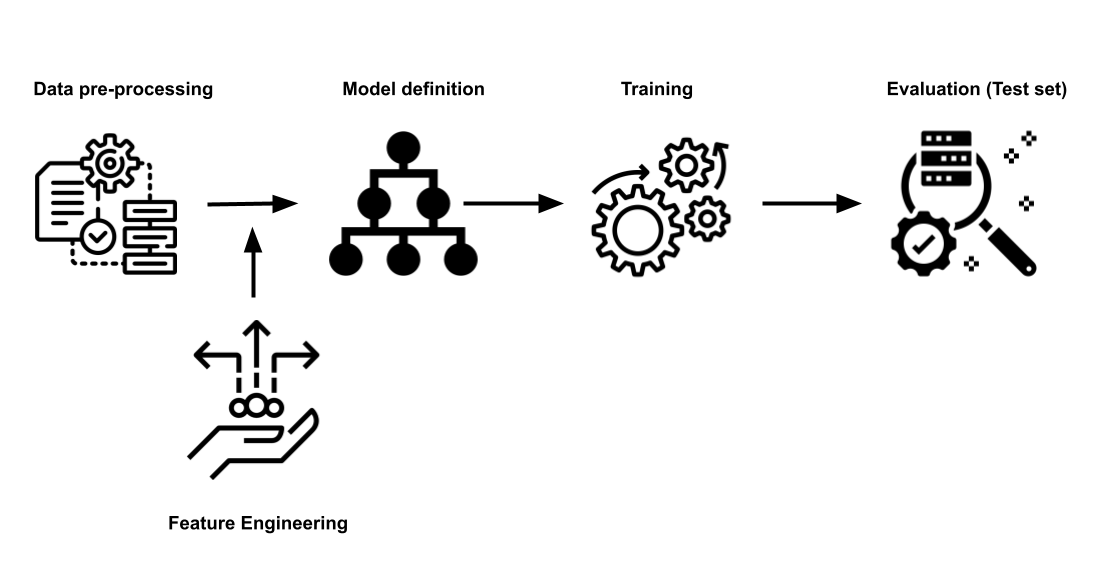
\includegraphics[width=0.7\textwidth]{thesis/Baseline_pipeline.png}
    \caption{feature-based approach pipeline}
    \label{fig:feature-based approach pipeline}
\end{figure}

\subsection{Feature based approach}
In order to answer the second question and evaluate the fine-tuning based approach, baselines have been trained using selected features. For this, convolutional neural network (CNN) model for text classification has been trained using Glove (global vectors for word representation) \cite{pennington2014glove}, Fasttext  \cite{joulin2017bag} and flair  \cite{akbik2019flair} pretrained word embeddings as features. Other models such as support vector machines with manually selected features, Multinomial naive Bayes model with term frequency - inverse document frequency (TF-IDF) and bag of words (BOW) have also been trained. Models which inherently support multi-label classification such as K-nearest neighbors classifier, decision tree classifier and random forest classifier with TF-IDF and BOW features have also been experimented.

The baseline models have been trained on the train, validation set used for training the language models and tested on the same test split with similar evaluation metrics, for fair comparison. The training pipeline followed for the feature based approach is shown in the figure \ref{fig:feature-based approach pipeline}. During the pre-processing step, the input data has been cleaned (removing tokens that are not alphabetic), lower cased and  lemmatized to its base form with and without stop words using spacy\footnote{\url{https://spacy.io/}}. 


In the feature engineering  step, the input data is being vectorized using different features in order to feed it to the model. For CNN; Glove (6Billion tokens,100 dimensional \footnote{\url{https://nlp.stanford.edu/projects/glove/}}), fasttext (Wiki-news-300 dimensional \footnote{\url{https://fasttext.cc/docs/en/pretrained-vectors.html}}) and flair (4098 dimensional \footnote{\url{https://github.com/flairNLP/flair}}) pre-trained embeddings models were used as features. Keras tokenizer \footnote{\url{https://www.tensorflow.org/api_docs/python/tf/keras/preprocessing/text/Tokenizer}} has been used to turn the lemmatized text into tokens with corresponding token\_ids. These token ids would be used as index to access the corresponding token (word to index mapping). After turning the lemmatized input text sequences to sequences of ids, the sequences are padded to fixed length. Then, the pre-trained word embeddings are extracted along with their corresponding word ids. Finally, a Keras embedding layer \footnote{\url{https://www.tensorflow.org/api_docs/python/tf/keras/layers/Embedding}} of features corresponding to the word embedding model is created by extracting the word embeddings corresponding to the ids of the lemmatized input text sequence. The embedding layer has shape of (v-vocab created by tokenizer, D-word embedding dimension). The same tokenizer is used, and the same methodology is followed for the three word embedding models to have a fair comparison of results. Coming to the machine learning models, selected lexical and syntactic features  mainly form the paper \cite{recasens2013linguistic}  have been used along with TF-IDF and BOW features. The list of selected features can be seen in the table \ref{tab:features}. The table shows the feature name with value and type and small description about the feature. There are two types of features, count based features which are purely based on count and score based features which are calculated based on some formula. Coming to score based features, flesch readability score \cite{flesch1948new} using textstat library \footnote{\url{https://textstat.readthedocs.io/en/latest/}} is used to determine the readability and test whether stereotypes are explicit/overt or subtle, subjectivity score using textblob \footnote{\url{https://textblob.readthedocs.io/en/dev/}} is used to determine whether stereotypes are subjective in nature, sentiment analysis using vader sentiment analysis library \footnote{\url{https://github.com/cjhutto/vaderSentiment}} with positive, negative, neutral scores have been used to determine sentiment of stereotypes. Average word length, max\_tf\_idf scores have also been used to gather general text statistics. 

% Please add the following required packages to your document preamble:
% \usepackage{booktabs}
% \usepackage{graphicx}
\begin{table}[]
\resizebox{\textwidth}{!}{%
\begin{tabular}{@{}llll@{}}
\toprule
Id & Feature                  & Value                                   & Description                                                \\ \midrule
1  & Flesch\_score            & \textless{}Numeric, score\textgreater{} & Reading ease of the stereotype sample                      \\
2  & Subjectivity\_score      & \textless{}Numeric, score\textgreater{} & Subjectivity of stereotype sample                          \\
3  & Neg                      & \textless{}Numeric, score\textgreater{} & Negative score of stereotype sample                        \\
4  & Pos                      & \textless{}Numeric, score\textgreater{} & Positive score of stereotype sample                        \\
5  & Neu                      & \textless{}Numeric, score\textgreater{} & Neutral score of stereotype sample                         \\
6  & Num\_chars               & \textless{}Numeric, count\textgreater{} & Number of characters in stereotype sample                  \\
7  & Num\_words               & \textless{}Numeric, count\textgreater{} & Number of words in stereotype sample                       \\
8  & Avg\_word\_length        & \textless{}Numeric, score\textgreater{} & Average number of words in stereotype sample               \\
9  & Max\_tf\_idf\_feature    & \textless{}Numeric, score\textgreater{} & Maximum TF-IDF score of stereotype sample                  \\
10 & Assertive\_verbs\_count  & \textless{}Numeric, count\textgreater{} & Number of Assertive verbs in stereotype sample             \\
11 & Factive\_verb\_count     & \textless{}Numeric, count\textgreater{} & Number of factive verbs in stereotype sample               \\
12 & Hedges\_count            & \textless{}Numeric, count\textgreater{} & Number of hedges in stereotype samples                     \\
13 & Implicative\_verb\_count & \textless{}Numeric, count\textgreater{} & Number of implicative verbs in stereotype sample           \\
14 & SubjectivityClues\_lexicon\_count        & \textless{}Numeric, count\textgreater{} & Number of subjectivity clues in stereotype sample                           \\
15 & Bias\_word\_list\_01\_2018\_count        & \textless{}Numeric, count\textgreater{} & Number of bias words in stereotype sample                                   \\
16 & NNS\_count               & \textless{}Numeric, count\textgreater{} & Number of plural nouns in stereotype sample                \\
17 & NNPS\_count              & \textless{}Numeric, count\textgreater{} & Number of proper plural nouns in stereotype sample         \\
18 & DT\_count                & \textless{}Numeric, count\textgreater{} & Number of determiners in stereotype sample                 \\
19 & JJ\_count                & \textless{}Numeric, count\textgreater{} & Number of adjectives in stereotype sample                  \\
20 & JJS\_count               & \textless{}Numeric, count\textgreater{} & Number of superlative adjectives in stereotype sample      \\
21 & NN\_count                & \textless{}Numeric, count\textgreater{} & Number of nouns in stereotype sample                       \\
22 & Adverb\_count            & \textless{}Numeric, count\textgreater{} & Number of adverbs in stereotype sample                     \\
23 & NORP\_count                              & \textless{}Numeric, count\textgreater{} & Number of nationality or religious or political groups in stereotype sample \\
24 & PERSON\_count            & \textless{}Numeric, count\textgreater{} & Number of people, including fictional in stereotype sample \\
25 & GPE\_count               & \textless{}Numeric, count\textgreater{} & Number of countries, cities, states in stereotype sample   \\
26 & Characteristic\_terms\_ethnicity\_count  & \textless{}Numeric, count\textgreater{} & Number of characteristic ethnicity terms in stereotype sample               \\
27 & Characteristic\_terms\_profession\_count & \textless{}Numeric, count\textgreater{} & Number of characteristic profession terms in stereotype sample              \\
28 & Characteristic\_terms\_gender\_count     & \textless{}Numeric, count\textgreater{} & Number of characteristic gender terms in stereotype sample                  \\
29 & Characterisitc\_terms\_religion\_count   & \textless{}Numric, count\textgreater{}  & Number of characteristic religion terms in stereotype sample                \\ \bottomrule
\end{tabular}%
}
\caption{Manually selected features for SVM baseline}
\label{tab:features}
\end{table}

Coming to the count based features, lexicons gathered from the paper  \cite{recasens2013linguistic}  have been used as count based features as described in the table \ref{tab:features}. The lexical features were used to test whether a sentence is biased or not. Coming to linguistic features [10-14 in table], Assertive verbs \cite{hooper1975assertive} are the verbs whose "complement clauses assert certainty of proposition"\cite{recasens2013linguistic}. For e.g. verbs such as "point out" and "claim" cast doubt on the certainty of the proposition than verbs such as "say" and "state" \cite{recasens2013linguistic}. Factive verbs \cite{kiparsky1970progress} are the verbs that "pre-suppose the truth of their complement clause "\cite{recasens2013linguistic} for e.g. "He realized" and "reveal" presuppose the truth rather than  "his stand" and "indicated". Hedges are the words which used to avoid bold predictions or statements. E.g. words such as "may", "possibly" \cite{recasens2013linguistic}. Implicative verbs \cite{karttunen1971implicative} are the verbs "which implies truth or untruth of the complement depending on polarity"\cite{recasens2013linguistic}. E.g. verbs such as "murdered" with negative polarity, "coerced into accepting" with negative polarity than "killed" or "accepting". Overall, these linguistic features indicate bias in the proposition. Strong subjectivity words are extracted from subjectivity clues lexicon \cite{wilson2005recognizing} to determine the subjectivity involved in stereotypes. Parts of speech tags and Named entity recognition (NER) tags were created for the lemmatized input sentences using spacy  library. Tags such as NNS (Plural nouns), NNPS (Proper plural nouns) were used to determine the generalization involved in stereotype sample. Tags JJ(Adjective), JJS(superlative adjectives) were used to indicate attribute terms and superlative adjectives to indicate subjectivity. Tags DT (Determiner) were used due to the high presence of "The" with people found in EDA report, which indicate generalization. Tag RB (adverb) to indicate generic sentences where frequency adverb (usually, typically, generally, sometimes, always) are used. Coming to NER tags, NORP (Nationalities or religious groups or political groups), GPE (Countries, cities, states) were used as a cue to detect ethnic groups. Finally, the top thousand characteristic terms based on scaled F-score (harmonic mean of precision and recall with scaling factor) from ethnicity, gender, profession, religion bias groups were extracted using scattertext \footnote{\url{https://github.com/JasonKessler/scattertext}} to presence of indicate different bias type.

Coming to the model definition step, the CNN model was created and trained using Keras library \footnote{\url{https://keras.io/}}. The basic architecture of CNN model used is embedding layer followed by 1D convolutional layer with 128 filters to extract features with a kernel size of 3 followed by maxpooling1D with pool size of 3 to extract the maximum value over the window. This setup is repeated for three times followed by a globalMaxpool1D to get overall important features and finally a dense output layer with output size corresponding to number of labels (in our case 7). Sigmoid activation function and binary cross entropy loss function is used as we are dealing with multi label classification. Multinomial Naive Bayes and support vector machines (SVM) along with others were created and trained using scikit learn library \footnote{\url{https://scikit-learn.org/stable/}}. The important step is that Multinomial Naive Bayes and SVM don't inherently support multi label classification, hence MultiOutputClassifier \footnote{\url{https://scikit-learn.org/stable/modules/generated/sklearn.multioutput.MultiOutputClassifier.html#sklearn.multioutput.MultiOutputClassifier}} is used where one classifier is fit to each label to support multi label classification following the binary relevance transformation method.

Coming to the training, in the case of CNN model with different word embedding features, the models were  trained for 40 epochs, with a batch size of 128. Early stopping callback is used with patience set to 5.
Early stopping is a technique used to stop training by monitoring a metric, (goal to minimize validation loss in our case) if there is no longer an improvement. Patience parameter is used to Waite for n epochs before stopping the training. Coming to machine learning models, the classifier models wrapped with multi output classifier method along with other classifiers were fitted to train set (combination of train and validation splits). Finally, all the models are tested on the same test set used for testing the language models for fair comparison.

\subsubsection{Brief description of models}
\textbf{------------------TBD------------------------------------------------}


Coming to the deep learning models, convolutional neural network has been chosen to experiment with because, CNN can be a much faster alternative to recurrent neural networks for tasks like text classification. 
\begin{enumerate}
    \item How does accuracy vary with non-contextual word embeddings (e.g. Glove, Word2Vec) to BERT word embedding?
    \item How does accuracy vary with baseline architecture (applying word embeddings to sentence and taking arithmetic average) to a fine-tuned BERT model ?
\end{enumerate}

    \begin{itemize}
        \item Lexicon - based approach : 
        \begin{itemize}
            \item Project into word embedding space and score each word based on its distance from woman, men ??
            \textbf{Refer }\cite{cryan2020detecting}
        \end{itemize}
        \item Brief description of  models and features
        \begin{itemize}
            \item SVM with selected lexicons + different features (toxicity, sentiment)
            \item Text-CNN with GLove,flair embedding
            \item Random embedding with GRU and LSTM 
        \end{itemize}
        \begin{itemize}
            \item Lexicons, POS and NER tags 
            \begin{itemize}
                \item Generalization : Plural nouns (NNS,NNPS), articles, article(the) + adjective(Refer to the whole group), determiner, quantifier (many,few, several...), frequency adverbs (Generic sentences - usually, typically, generally, sometimes, always)
                \item Subjectivity : strong subjectivity lexicon \cite{tangpersonalized}
                \item Syntactic cues : Syntactic negation (describing Stereotype-inconsistent )
            \end{itemize}
        \end{itemize}
        \item Why these model?
    \end{itemize}
\textbf{------------------TBD------------------------------------------------}
\section{Evaluation metrics}
Evaluation of multi label classification problem is much complicated than traditional single label setting, as an example can be associated to multiple labels and the predictions of the learned model could be partially correct\cite{sorower2010literature}\cite{zhang2013review}. Hence, there arises a number of evaluation metrics that can be used to capture different notions. 
Broadly, the evaluation metrics used for multi-label classification can be categorized into two groups, namely example or sample based metrics and label based metrics \cite{zhang2013review}.
% \cite{tsoumakas2007multi}
\subsection{Example or sample based metrics}
Example based metrics evaluate the learned model on each test sample separately and returns the mean over the test set\cite{zhang2013review}. The following sample or example based metrics have been evaluated.

\subsubsection{Subset accuracy or Exact match ratio}

 $$\frac{1}{n}\sum_{i =1}^{n}[h(x_i) == Y_i]$$
 
\subsubsection{Hamming loss}
\subsubsection{Hamming score / Accuracy}
\subsubsection{Precision}
\subsubsection{Recall}
\subsubsection{F-Measure}

\subsection{Label based metrics}
Label based metrics evaluate the learned model on each class label separately and average(micro/macro) over all the class labels \cite{zhang2013review}. 
    
\subsubsection{Macro average}

\subsubsection{Micro average}

\\
\\
Label based methods would fail to directly address the correlation among different classes, as the order of classes are not taken into consideration\cite{zhang2010multi}. Hence, sample based metrics are used as main evaluation metric in this thesis.